\documentclass{standalone}

\usepackage{tikz}

\usetikzlibrary{shapes.geometric, arrows}
\usepackage{amsmath}

\tikzstyle{arrow} = [-stealth]
\begin{document}
    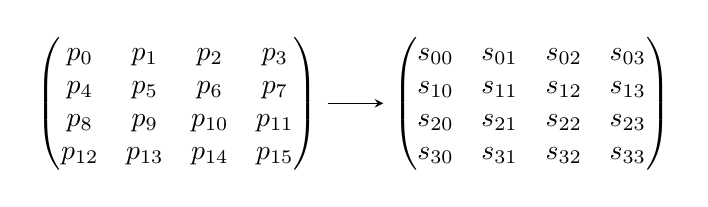
\begin{tikzpicture}
        \node [rectangle] (ptx) {
            $\begin{pmatrix}
                p_0 & p_1 & p_2 & p_3 \\
                p_4 & p_5 & p_6 & p_7 \\
                p_8 & p_9 & p_{10} & p_{11} \\
                p_{12} & p_{13} & p_{14} & p_{15}
            \end{pmatrix}$
        };
        \node [rectangle, right of=ptx, node distance=4.5cm] (state) {
            $\begin{pmatrix}
                s_{00} & s_{01} & s_{02} & s_{03} \\
                s_{10} & s_{11} & s_{12} & s_{13} \\
                s_{20} & s_{21} & s_{22} & s_{23} \\
                s_{30} & s_{31} & s_{32} & s_{33}
            \end{pmatrix}$
        };
        \draw [arrow] (ptx) -- (state);
    \end{tikzpicture}
\end{document}